\documentclass[twoside]{article}
\setlength{\oddsidemargin}{0.25 in}
\setlength{\evensidemargin}{-0.25 in}
\setlength{\topmargin}{-0.6 in}
\setlength{\textwidth}{6.5 in}
\setlength{\textheight}{8.5 in}
\setlength{\headsep}{0.75 in}
\setlength{\parindent}{0 in}
\setlength{\parskip}{0.1 in}

%
% ADD PACKAGES here:
%

\usepackage{amsmath,amsfonts,graphicx,mathdots}
\usepackage{tcolorbox}
\usepackage{enumitem}

\newcounter{lecnum}
\renewcommand{\thepage}{\thelecnum-\arabic{page}}
\renewcommand{\thesection}{\thelecnum.\arabic{section}}
\renewcommand{\theequation}{\thelecnum.\arabic{equation}}
\renewcommand{\thefigure}{\thelecnum.\arabic{figure}}
\renewcommand{\thetable}{\thelecnum.\arabic{table}}
\newcommand{\N}{\operatorname{\mathcal{N}}}
\renewcommand{\t}{^\mathrm{T}{}}
\newcommand{\E}{\mathrm{E}{}}
\newcommand{\tr}{\mathrm{tr}{}}
\renewcommand{\k}{_k{}}
\newcommand{\kp}{_{k+1}{}}
\newcommand{\kpk}{_{k+1\mid k}{}}
\newcommand{\kpkp}{_{k+1\mid k+1}{}}
\newcommand{\kk}{_{k\mid k}{}}
\DeclareMathOperator*{\argmin}{argmin}

%
% The following macro is used to generate the header.
%
\newcommand{\lecture}[4]{
   \pagestyle{myheadings}
   \thispagestyle{plain}
   \newpage
   \setcounter{lecnum}{#1}
   \setcounter{page}{1}
   \noindent
   \begin{center}
   \framebox{
      \vbox{\vspace{2mm}
    \hbox to 6.28in { {\bf EE402 - Discrete Time Systems
	\hfill Fall 2021} }
       \vspace{4mm}
       \hbox to 6.28in { {\Large \hfill Lecture #1 \hfill} }
       \vspace{2mm}
       \hbox to 6.28in { {\it Lecturer: #2 \hfill } }
      \vspace{2mm}}
   }
   \end{center}
   \markboth{Lecture #1}{Lecture #1}

   \vspace*{4mm}
}

\renewcommand{\cite}[1]{[#1]}
\def\beginrefs{\begin{list}%
        {[\arabic{equation}]}{\usecounter{equation}
         \setlength{\leftmargin}{2.0truecm}\setlength{\labelsep}{0.4truecm}%
         \setlength{\labelwidth}{1.6truecm}}}
\def\endrefs{\end{list}}
\def\bibentry#1{\item[\hbox{[#1]}]}


\newcommand{\fig}[3]{
			\vspace{#2}
			\begin{center}
			Figure \thelecnum.#1:~#3
			\end{center}
	}

% Use these for theorems, lemmas, proofs, etc.
\newtheorem{theorem}{Theorem}[lecnum]
\newtheorem{lemma}[theorem]{Lemma}
\newtheorem{proposition}[theorem]{Proposition}
\newtheorem{claim}[theorem]{Claim}
\newtheorem{corollary}[theorem]{Corollary}
\newtheorem{definition}[theorem]{Definition}
\newenvironment{proof}{{\bf Proof:}}{\hfill\rule{2mm}{2mm}}

% **** IF YOU WANT TO DEFINE ADDITIONAL MACROS FOR YOURSELF, PUT THEM HERE:

\begin{document}

% Lecture Details
\lecture{18}{Elif Sarıtaş}

\par

\section*{Preliminaries}

\subsection*{Multivariate Normal Distribution}
A multivariate normal distribution for $x\in\mathbb{R}^{n_x}$
\begin{align*}
	p(x) =& \N(x;\mu,\Sigma)\\
	=&\frac{1}{\sqrt{\textrm{det}(2\pi\Sigma)}} \exp\left\lbrace-\frac{1}{2}(x-\mu)\t\Sigma^{-1}(x-\mu) \right\rbrace 
\end{align*}
where 
\begin{align*}
	\mu =& \E\left[x \right] \\
	\Sigma =& \E\left[(x-\mu)(x-\mu)\t \right] \\
\end{align*}
Remember that any covariance matrix is
\begin{enumerate}[label=\roman*.]
	\item a square matrix (in this case $\Sigma \in \mathbb{R}^{n_x\times n_x}$)
	\item symmetric, i.e., $\Sigma = \Sigma\t$
	\item positive semi-definite, i.e., $a\t\Sigma a \geq 0,\hspace{0.2cm}\forall a$
\end{enumerate}
\paragraph{Marginal Distribution:}
Given that $x\sim\N(x;\mu,\Sigma)$ where
$x = \left[\begin{array}{cc}
		x_a & x_b
	\end{array} \right]\t$, $
	\mu = \left[\begin{array}{cc}
		\mu_a & \mu_b
	\end{array} \right]\t $, and $
	\Sigma = \left[\begin{array}{cc}
		\Sigma_a & \Sigma_c\\
		\Sigma_c & \Sigma_b
	\end{array} \right] $, then
\begin{align*}
	p(x_a) =& \N(x_a;\mu_a,\Sigma_a)\\
	p(x_b) =& \N(x_b;\mu_b,\Sigma_b)
\end{align*}


\paragraph{Conditional Distribution:}
Given that $x\sim\N(x;\mu,\Sigma)$ where
$x = \left[\begin{array}{cc}
	x_a & x_b
\end{array} \right]\t$, $
\mu = \left[\begin{array}{cc}
	\mu_a & \mu_b
\end{array} \right]\t $, and $
\Sigma = \left[\begin{array}{cc}
	\Sigma_a & \Sigma_c\\
	\Sigma_c & \Sigma_b
\end{array} \right] $, then
\begin{align*}
	p(x_a\mid x_b) =& \N(x_a;\mu_{a\mid b},\Sigma_{a\mid b})\\
\end{align*}
where
\begin{align*}
	\mu_{a \mid b} =& \mu_a + \Sigma_c \Sigma_b^{-1}(x_b-\mu_b)\\
	\Sigma_{a \mid b} =& \Sigma_a - \Sigma_c\Sigma_b^{-1}\Sigma_c\t 
\end{align*}
\paragraph{Linear Combinations:}
Linear combinations of jointly Gaussian densities are also Gaussian, which is one of the main reasons for Gaussian densities being this popular. Given two jointly normal random variables, $(x,y)\sim\N\left( \left[ \begin{array}{c}
	x\\y
\end{array}\right] ;\left[ \begin{array}{c}
\mu_x\\\mu_y
\end{array},\right],\left[ \begin{array}{cc}
\Sigma_x & \Sigma_{xy}\\ \Sigma_{y} & \Sigma_{yx}
\end{array}\right]\right)   $, then 
\begin{align*}
	z =& Ax+By+c \\
	z \sim& \N(z;A\mu_x+B\mu_y+c,A\Sigma_xA\t+B\Sigma_yB\t+A\Sigma_{xy}B\t+B\Sigma_{yx}A\t)
\end{align*}
When $x$ and $y$ are independent, $\Sigma_{xy}=0$, then covariance matrix of the $z$ becomes
\begin{align*}
	z \sim& \N(z;A\mu_x+B\mu_y+c,A\Sigma_xA\t+B\Sigma_yB\t)
\end{align*}
\subsection*{Markov Property}
A process, $x$, is called is Markov, if
\begin{align*}
	p(x\k \mid x_{k-1},x_{k-2},\cdots,x_0) = p(x\k \mid x_{k-1})\hspace{0.2cm}\forall k.
\end{align*}
That is the transition between the states depend only on the previous state, which is a summary of the past.

\subsection*{Estimators}
An estimator is an algorithm to find one or more unknown values using observations. These unknowns may be 
\begin{itemize}
	\item stochastic or deterministic, 
	\item static or dynamic,
	\item finite dimensional or infinite dimensional.
\end{itemize}
There are three inference problems in the Bayesian framework. 

	\paragraph{\textbf{Prediction}:} In this problem, the estimate of an $n$-step ahead future state is computed by considering the measurements up to time $k$. That is we deal with the following distribution
	\begin{align*}
		p(x_{k+n}\mid Y_k),\hspace{0.2cm} \textrm{where} \hspace{0.2cm}n=1,2,\cdots
	\end{align*}
	\paragraph{\textbf{Filtering}:} In this case, we estimate the state at time $k$ using the measurements up to and including the time $k$. The distribution we consider is 
	\begin{align*}
		p(x_{k}\mid Y_k),\hspace{0.2cm} 
	\end{align*}
	\paragraph{\textbf{Smoothing}:}This time all of the measurements in an interval is used to estimate the state at a time instant in that interval. Hence, the distribution of interest is now
	\begin{align*}
		p(x_{k}\mid Y_T),\hspace{0.2cm}\hspace{0.2cm} \textrm{where} \hspace{0.2cm}k<T,\cdots
	\end{align*}

\begin{figure}[!h]
	\centering
	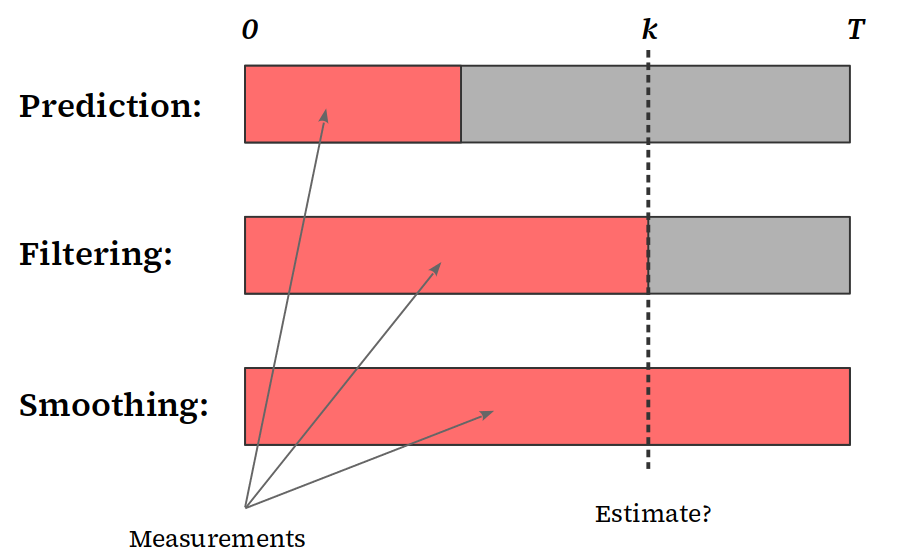
\includegraphics[trim={0cm 0cm 0cm 0cm},clip,width=0.5\textwidth]{figures/inference}
	\caption{Inference problems (Courtesy of Murat Kumru)}
	\label{fig:Inference}
\end{figure}

\subsubsection*{Minimum Mean Square Error}
Mean square error (MSE) is a measure that demonstrates how much estimates deviate from their true values. It is used as an performance indicator for estimators, and it is defined as
\begin{align*}
	\textrm{MSE}_\theta = \E\left[(\theta-\hat \theta)\t(\theta-\hat \theta) \right]  
\end{align*}
where $\theta \sim p(\theta)$,  and  $\hat\theta$ is the estimate.Minimum mean square error is the estimator that minimizes MSE. 

\newpage

\section*{Discrete-Time Kalman Filter}
\subsection*{Problem Definition}
We consider a linear-Gaussian system, in which the models are linear and the noise characteristics are Gaussian.
\begin{align*}
	x\kp &= G x\k + H u\k + w\k
	\\
	y\k &= C x\k + v\k
\end{align*}
where 
\begin{itemize}
	\item $x\k \in \mathbb{R}^{n_x}$ is the state,
	\item $y\k \in \mathbb{R}^{n_x}$ is the measurement,
	\item $w\k \in \mathbb{R}^{n_x}$ is the process noise with $w\k \sim \mathcal{N}(w\k;0,Q)$,
	\item $v\k \in \mathbb{R}^{n_x}$ is the measurement noise with $v\k \sim \mathcal{N}(v\k;0,R)$,
	\item $u\k$ is either deterministic or known, it may a function of known variables.
	
	\item We denote all of the measurements collected from the start up to  and including the time k as $Y\k = \left\lbrace y_0, y_1, \cdots,y_k \right\rbrace$.
\end{itemize}
The process noise captures the uncertainties regarding the system dynamics, whereas the measurements noise depends on the noise characteristics of the sensors. The probabilistic model for this system is written as
\begin{align*}
	p(x\kp\mid x\k) =& \N(x\kp;Gx\k+Hu\k,Q),\\
	p(y\k\mid x\k) =& \N(y\k;Cx\k,R).
\end{align*}
This system can be modelled using block diagrams as follows.
\begin{figure}[!h]
	\centering
	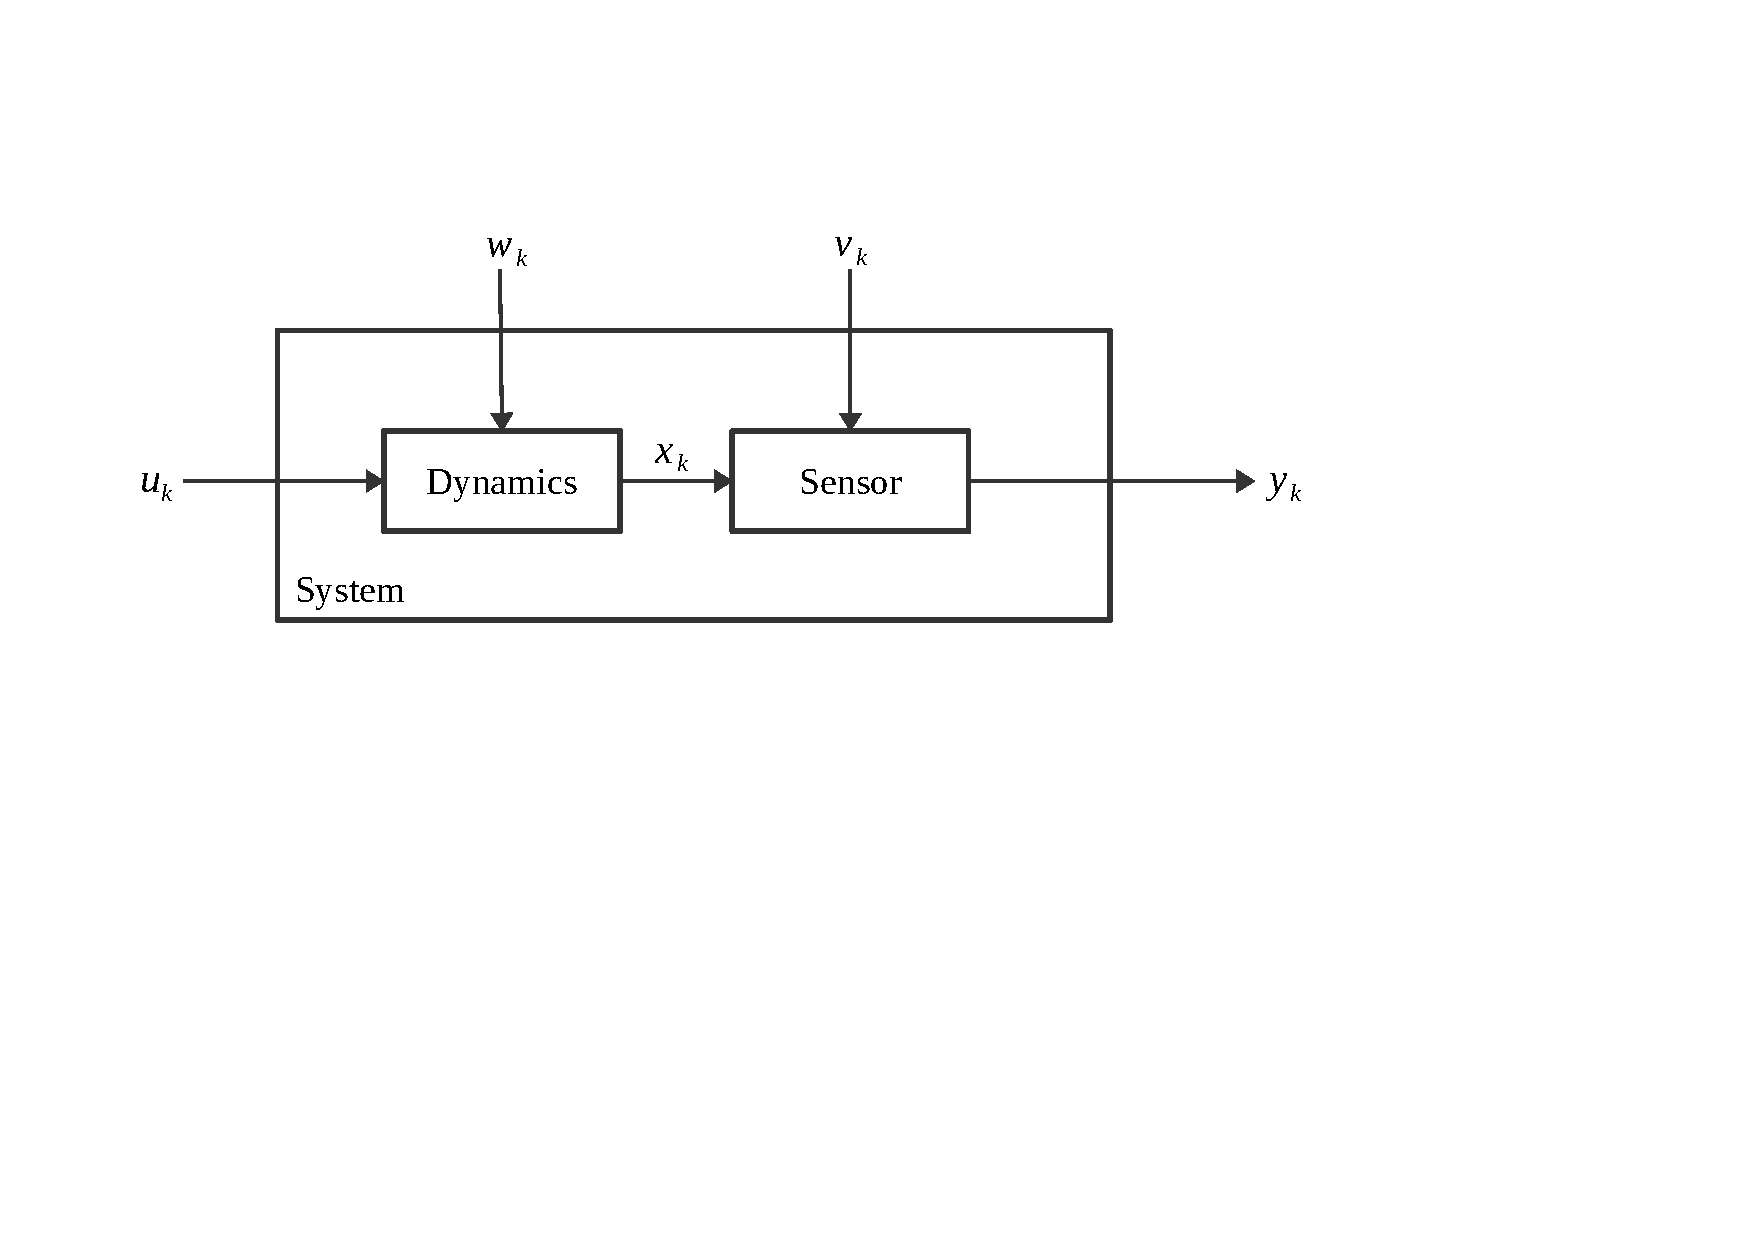
\includegraphics[trim={1cm 10cm 7cm 4cm},clip,width=0.75\textwidth]{figures/system}
	\caption{Block diagram of the system}
	\label{fig:system}
\end{figure}


The initial state is distributed according to
\begin{align*}
	x_0 \sim \N(x_0;\hat x_{0\mid0},P_{0\mid0}).
\end{align*}

We assume that $x_0$, $w_0$,  $w_1$,  $\cdots$ and $v_0$, $v_1$, $\cdots$ are  independent.

\textbf{Goal:} Given the measurements $y_0$, $y_1$, $\cdots$, $y_k$, find an estimate of $x\k$ such that the loss function, $\E\left[(x\k-\hat x\k)\t(x\k-\hat x\k) \right] $, is minimized.

\subsubsection*{Notation}
We will use the following notations throughout the derivation, the first one of the densities below is called the predicted density, whereas the latter is the posterior density.

\begin{align*}
	p(x\kp\mid Y\k) =& \N(x\kp; \hat x\kpk,P\kpk)\\
	p(x\k\mid Y\k) =& \N(x\k; \hat x\kk,P\kk)\\
\end{align*}
\begin{tcolorbox} [colback=blue!5!white,colframe=blue!75!black,title=\textbf{Remark}:,subtitle style={boxrule=0.4pt,
		colback=yellow!50!red!25!white}]
	If we can find a linear estimator, the above equations will hold; as the linear combinations of independent Gaussians are also Gaussian.
\end{tcolorbox}

\subsection*{Derivation}

Let us first consider the prediction problem, as it is quite simple given the motion model. The prediction problem aims to find $\E\left[x\kp \mid Y\k \right] $. 
\begin{align*}
	\hat{x}\kpk =& \E\left[x\kp \mid Y\k \right]\\
	 =& \E\left[G x\k + H u\k + w\k \mid Y\k \right]\\
	=& \E\left[G x\k \mid Y\k \right] + \E\left[H u\k \mid Y\k \right] + \E\left[w\k \mid Y\k \right]\\
	=& G\E\left[x\k \mid Y\k \right] + H u\k \\
	=& G \hat x\kk + H u\k
\end{align*} 
Note that the input, $u\k$, is deterministic and $\E\left[w\k \mid Y\k \right]=\E\left[w\k \right]=0 $.

The predicted error covariance is defined and computed as
\begin{align*}
	P\kpk =& \E\left[(x\kp-\hat x\kpk)(x\kp-\hat x\kpk)\t \mid Y\k \right]\\
	=& \E\left[(G x\k + H u\k + w\k- G \hat x\kk - H u\k)(G x\k + H u\k + w\k- G \hat x\kk - H u\k)\t \mid Y\k \right]\\
	=& \E\left[\big(G (x\k-\hat x\kk) + w\k\big)\big(G (x\k-\hat x\kk) + w\k\big)\t \mid Y\k \right]\\
	=& G\E\left[(x\k-\hat x\kk)(x\k-\hat x\kk)\t \mid Y\k \right]G\t +  \E\left[ w\k w\k\t \mid Y\k \right] \\
	=& G P \kk G\t + Q
\end{align*} 
where we use the fact that $\E\left[ w\k w\k\t \mid Y\k \right] = Q$.

\begin{tcolorbox} [colback=blue!5!white,colframe=blue!75!black,title=\textbf{Remark}:,subtitle style={boxrule=0.4pt,
		colback=yellow!50!red!25!white}]
Both the predicted state and the predicted error covariance estimates depend on the filtered estimates on the previous time step.
\end{tcolorbox}

Now in order to find the filter estimates at time $k+1$, the idea is to use the predicted estimates and incorporate the new measurement arriving at time $k+1$ into the procedure. Thus, we start this part of the derivation by making the guess that the filtered state estimate is a linear combination of the predicted state and the additional information obtained from the new measurement. That is
\begin{align*}
	\hat x\kpkp = \hat x\kpk + K\kp (y\kp - \hat y\kpk)
\end{align*}
where $\hat y \kpk$ is the predicted measurement,
\begin{align*}
	\hat y \kpk = C \hat x \kpk,
\end{align*}
the predicted measurement error is named as innovation, and $K$ is an unknown matrix named as Kalman gain. We wish to determine the Kalman gain such that the loss function is minimized. Then,
\begin{align*}
	\hat x\kpkp =& \hat x\kpk + K\kp (Cx\kp + v\kp - C \hat x \kpk)\\
	P\kpkp =& \E\left[(x\kp-\hat x\kpkp)(x\kp-\hat x\kpkp)\t\right] \\
	=& \E\left[\big(x\kp-\hat x\kpk - K\kp (Cx\kp + v\kp - C \hat x \kpk)\big)\right. \\
	&\left. \big(x\kp-\hat x\kpk - K\kp (Cx\kp + v\kp - C \hat x \kpk)\big)\t  \right]\\
	=& \E\left[\big((I-K\kp C)(x\kp-\hat x\kpk) - K\kp v\kp\big) \big((I-K\kp C)(x\kp-\hat x\kpk) - K\kp v\kp\big)\t \right]\\
	=& (I-K\kp C)\E\left[(x\kp-\hat x\kpk) (x\kp-\hat x\kpk)\t \right](I-K\kp C)\t + K\kp\left[v\kp v\kp\t \right] K\kp\t\\
	& -2\E\left[K\kp v\kp(x\kp-\hat x\kpk)\t(I-K\kp C)\t \right] \\
	=& (I-K\kp C)P\kpk(I-K\kp C)\t + K\kp RK\kp \t\\
	=& P\kpk + K\kp C P\kpk C\t K\kp\t - K\kp C P\kpk - P\kpk C\t K\kp\t + K\kp RK\kp \t
\end{align*}

Remember that our aim is to find the Kalman gain that minimizes the loss function, i.e.,
\begin{align*}
	K\kp = \underset{K}{\argmin} \E\left[(x\kp-\hat x\kpkp)\t(x\kp-\hat x\kpkp) \right] 
\end{align*}
We observe that loss function is equivalent to the trace of the filtered error covariance.
\begin{align*}
	\E\left[(x\kp-\hat x\kpkp)\t(x\kp-\hat x\kpkp) \right]  = \tr\left[ P\kpkp\right] 
\end{align*}
Therefore, instead of minimizing the loss function we can minimize the trace of the filtered error covariance. For that purpose, we take the derivative of it with respect to the Kalman gain and set it to zero.
\begin{align*}
	\frac{\partial \tr\left[ P\kpkp\right] }{\partial K\kp } =& 2K\kp (C P\kpk C\t + R) - 2P\t\kpk C\t\\
	=& 0\\
	K\kp =& P\kpk C\t (C P\kpk C\t + R)^{-1}\\
	=& P\kpk C\t S^{-1}\kpk
\end{align*}
We substitute the gain into the update equations
\begin{align*}
	\hat x\kpkp =& \hat x\kpk + P\kpk C\t S^{-1}\kpk\kp (y\kp - \hat y\kpk)\\
	P\kpkp =& P\kpk - P\kpk C\t (CP\kpk C\t + R)^{-1} C P\kpk\\
	=& (I - K\kp C)P\kpk
\end{align*}
\begin{tcolorbox} [colback=blue!5!white,colframe=blue!75!black,title=\textbf{Remark}:,subtitle style={boxrule=0.4pt,
		colback=yellow!50!red!25!white}]
	Both the filtered state and the filtered error covariance estimates depend on the predicted estimates on the previous time step.
\end{tcolorbox}
\newpage
\subsection*{Properties of the Kalman Filter}
\begin{enumerate}
	\item The Kalman filter is a recursive algorithm, which is an implication of the model obeying the Markov property. The recursion visits the prediction and measurement update stages one after another till the end.
\begin{tcolorbox} [colback=red!5!white,colframe=red!75!black,title=\textbf{Kalman Filter Recursion}:,subtitle style={boxrule=0.4pt,
		colback=yellow!50!red!25!white}]
Given the initial distribution $p(x_0) = \N(x_0;\hat x_{0\mid0},P_{0\mid0})$\\ 

Repeat for each k:
	\begin{itemize}
		\item Prediction Update
		\begin{align}
			\hat{x}\kpk =& G \hat x\kk + H u\k \\
			P\kpk =& G P \kk G\t + Q
		\end{align}
		\item Measurement Update
		\begin{align}
			\hat x\kpkp =& \hat x\kpk + K\kp (y\kp - \hat y\kpk)\label{eq:stateMeasurementUpdate}\\
			P\kpkp =& P\kpk - K\kp S\kpk K\t\kp 
		\end{align}
	where
	\begin{align}
		\hat y\kpk =& C x\kpk \\
		S\kpk =& CP\kpk C\t + R\\
		K\kp =& P\kpk C\t S^{-1}\kpk
	\end{align}
	\end{itemize}
	
\end{tcolorbox}

	\item The Kalman gain and the covariance update equations do not depend on the measurements, hence they can be calculated offline once the model is given.
	\item The sufficient statistics to describe a Gaussian distribution are the mean and the covariance. Using Kalman filter, we compute this statistics, thus we make not only point estimations but also produce probability desity function estimates.
	\item The Kalman filter is an optimal observer, you can see that \eqref{eq:stateMeasurementUpdate} has the same form of a Luenberger's observer. 
	\item When we believe that we know the system dynamics quite surely, we keep the process noise covariance matrix, $Q$, small. Then, the resulting Kalman gain becomes also small that the effect of measurements on the estimates are kept small. Similarly, we can infer that when $Q$ is high, the measurements are incorporated into the estimates to a bigger extent, as we have more trust on the measurements than the system model.
	\item When we think that our sensor is highly noisy, we set the measurement noise covariance, $R$, to a high value, as a result the Kalman gain gets smaller. Therefore, estimates mostly depend on the predictions. In the case of a smaller $R$, the measurements affect the estimates more due to having a larger Kalman gain.
\end{enumerate}

\textbf{Example:} 2-D random walk with scalar measurement.
Consider the following system
\begin{align*}
	x\kp =& \left[ \begin{array}{cc}
		1 & 0 \\ 0 & 1
	\end{array}\right] x\k + w\k\\
	y\k =& \left[\begin{array}{cc}
		1 & 1
	\end{array} \right]  + v\k
\end{align*}
where $w\k \sim \N(w\k;0,Q) $, $v\k \sim \N(v\k;0,0.4) $, and $x_{0\mid 0}\sim\N(x_0;0,\mathrm{I}_{2\times2 })$ with $Q = 0.1\cdot \mathrm{I}_{2\times2}$. Given the measurements $y_1 = 1$  and $y_2=-1.5$, compute the filtered mean and covariance estimates for the first two time instants.

\textbf{Solution:} 
\begin{itemize}
	\item When $k = 1$:
	
	Prediction Update:
	\begin{align*}
		x_{1\mid 0} =& G x_{0\mid 0}\\
		=& \left[ \begin{array}{cc}
			1 & 0 \\ 0 & 1
		\end{array}\right] \left[ \begin{array}{c}
		0 \\ 0
	\end{array}\right] \\
		=&\left[ \begin{array}{c}
			0 \\ 0
		\end{array}\right] \\
		P_{1\mid 0} =& G P_{0\mid 0} G\t + Q\\
		=& \left[ \begin{array}{cc}
			1 & 0 \\ 0 & 1
		\end{array}\right]\left[ \begin{array}{cc}
		1 & 0 \\ 0 & 1
	\end{array}\right]\left[ \begin{array}{cc}
	1 & 0 \\ 0 & 1
	\end{array}\right]+\left[ \begin{array}{cc}
	0.1 & 0 \\ 0 & 0.1
	\end{array}\right]\\
	=& \left[ \begin{array}{cc}
		1.1 & 0 \\ 0 & 1.1
	\end{array}\right]
	\end{align*}
	
	Measurement Update:
	\begin{align*}
		S_{1\mid 0} =& C P_{1\mid0}C\t+R\\
		=& \left[\begin{array}{cc}
			1 & 1
		\end{array} \right] \left[ \begin{array}{cc}
		1.1 & 0 \\ 0 & 1.1
	\end{array}\right]\left[ \begin{array}{c}
	1 \\ 1
	\end{array}\right] + 0.4\\
	 =& 2.5\\
	 K_1 =& P_{1\mid0}C\t S^{-1}_{1\mid0}\\
	 =&\frac{1}{2.5}\left[ \begin{array}{cc}
	 	1.1 & 0 \\ 0 & 1.1
	 \end{array}\right]\left[ \begin{array}{c}
	 1 \\ 1
	 \end{array}\right]\\
	=& \left[ \begin{array}{c}
		0.44 \\ 0.44
	\end{array}\right]\\
	\hat y_1 =& C x_{1\mid0}\\
	=& \left[\begin{array}{cc}
		1 & 1
	\end{array} \right] \left[ \begin{array}{c}
	0 \\ 0
	\end{array}\right] \\
	=& 0
\end{align*}
\begin{align*}
	x_{1\mid1} =& x_{1\mid0}+K_1(y_1-\hat y_1)\\
	=& \left[ \begin{array}{c}
		0 \\ 0
	\end{array}\right] + \left[ \begin{array}{c}
	0.44 \\ 0.44
	\end{array}\right] (1-0)\\
	 =&\left[ \begin{array}{c}
		0.44 \\ 0.44
	\end{array}\right]\\
	P_{1\mid 1} =& P_{1\mid 0} - K_1 S_{1\mid 0}K_1\t\\
	 =& \left[ \begin{array}{cc}
	 	1.1 & 0 \\ 0 & 1.1
	 \end{array}\right]-2.5\left[ \begin{array}{c}
	 0.44 \\ 0.44
	 \end{array}\right]\left[ \begin{array}{cc}
	 0.44 & 0.44
	\end{array}\right]\\
	=&	\left[ \begin{array}{cc}
		0.62 & -0.48 \\ -0.48 & 0.62
	\end{array}\right]
	\end{align*}
\item When $k = 2$:

Prediction Update:
\begin{align*}
	x_{2\mid 1} =& G x_{1\mid 1}\\
	=& \left[ \begin{array}{cc}
		1 & 0 \\ 0 & 1
	\end{array}\right] \left[ \begin{array}{c}
		0.44 \\ 0.44
	\end{array}\right] \\
	=&\left[ \begin{array}{c}
		0.44 \\ 0.44
	\end{array}\right] \\
	P_{2\mid 1} =& G P_{1\mid 1} G\t + Q\\
	=& \left[ \begin{array}{cc}
		1 & 0 \\ 0 & 1
	\end{array}\right]\left[ \begin{array}{cc}
		0.62 & -0.48 \\ -0.48 & 0.62
	\end{array}\right]\left[ \begin{array}{cc}
		1 & 0 \\ 0 & 1
	\end{array}\right]+\left[ \begin{array}{cc}
		0.1 & 0 \\ 0 & 0.1
	\end{array}\right]\\
	=& \left[ \begin{array}{cc}
		0.72 & -0.48 \\ -0.48 & 0.72
	\end{array}\right]
\end{align*}

	Measurement Update:
\begin{align*}
	S_{2\mid 1} =& C P_{2\mid1}C\t+R\\
	=& \left[\begin{array}{cc}
		1 & 1
	\end{array} \right] \left[ \begin{array}{cc}
		0.72 & -0.48 \\ -0.48 & 0.72
	\end{array}\right]\left[ \begin{array}{c}
		1 \\ 1
	\end{array}\right] + 0.4\\
	=& 0.88\\
	K_2 =& P_{2\mid1}C\t S^{-1}_{2\mid1}\\
	=&\frac{1}{0.88}\left[ \begin{array}{cc}
		0.72 & -0.48 \\ -0.48 & 0.72
	\end{array}\right]\left[ \begin{array}{c}
		1 \\ 1
	\end{array}\right]\\
	=& \left[ \begin{array}{c}
		0.27 \\ 0.27
	\end{array}\right]\\
	\hat y_2 =& C x_{2\mid1}\\
	=& \left[\begin{array}{cc}
		1 & 1
	\end{array} \right] \left[ \begin{array}{c}
		0.44 \\ 0.44
	\end{array}\right] \\
	=& 0.88
\end{align*}
\begin{align*}
	x_{2\mid2} =& x_{2\mid1}+K_2(y_2-\hat y_2)\\
	=& \left[ \begin{array}{c}
		0.44 \\ 0.44
	\end{array}\right] + \left[ \begin{array}{c}
		0.27 \\ 0.27
	\end{array}\right] (-1.5-0.88)\\
	=&\left[ \begin{array}{c}
		0.2 \\ 0.2
	\end{array}\right]\\
	P_{2\mid 2} =& P_{2\mid 1} - K_2 S_{2\mid 1}K_2\t\\
	=& \left[ \begin{array}{cc}
		0.72 & -0.48 \\ -0.48 & 0.72
	\end{array}\right]-0.88\left[ \begin{array}{c}
		0.27 \\ 0.27
	\end{array}\right]\left[ \begin{array}{cc}
		0.27 & 0.27
	\end{array}\right]\\
	=&	\left[ \begin{array}{cc}
		0.66 & -0.54 \\ -0.54 & 0.66
	\end{array}\right]
\end{align*}
\end{itemize}








% **** This ENDS THE EXAMPLES. DON'T DELETE THE FOLLOWING LINE:
\end{document}